\documentclass[20pt, a0paper, landscape]{tikzposter}

\usepackage{minted}

\usetheme{Simple}
\usetitlestyle{Filled}
\tikzposterlatexaffectionproofoff

\colorlet{titlefgcolor}{black}
\colorlet{titlebgcolor}{white}
\colorlet{blocktitlefgcolor}{blue!50!black}

\settitle{
  \begin{minipage}{0.5\linewidth}
    \color{titlefgcolor} {\bfseries \Huge \@title \par}
    \vspace*{1em}{\Large \@author \par}
  \end{minipage}
  \begin{minipage}{0.25\linewidth}
    \centering \color{titlefgcolor} \Large
    \texttt{https://github.com/lasp/hapi-server}
    \texttt{chris.lindholm@lasp.colorado.edu}
  \end{minipage}
  \begin{minipage}{0.25\linewidth}
    \raggedleft \@titlegraphic
  \end{minipage}
}

\title{A HAPI Service Interface for LaTiS}
\author{C. Lindholm, D. Lindholm, T. Baltzer}
\titlegraphic{
  
\includegraphics[scale=0.25]{img/lasp-logo}
}

\begin{document}
\maketitle[titletoblockverticalspace=0em]

  \begin{columns}
    \column{0.5}

    \begin{subcolumns}

      \subcolumn{0.5}
      \block{Overview}{
        \begin{itemize}
        \item The LASP HAPI server is a standalone data server
          implementing the Heliophysics Application Programmer’s
          Interface 2.0 specification (HAPI,
          \texttt{https://github.com/hapi-server/data-specification/}).
        \item HAPI is an interoperable, REST-style interface to
          timeseries data. It provides mechanisms for viewing a
          catalog of datasets, accessing dataset metadata, and
          streaming datasets subset both in time and parameters.
        \item Our server is built on LaTiS, a library for modeling and
          manipulating data using the functional data model. The
          functional data model is a specialization of the relational
          data model in which relations are strengthened to functions,
          providing richer semantics useful for representing
          scientific data.
        \item By building on LaTiS we can take advantage of existing
          adapters to data formats and datasets already modeled by
          LaTiS, including datasets from the LASP Interactive Solar
          Irradiance Datacenter (LISIRD,
          \texttt{http://lasp.colorado.edu/lisird}).
        \item Our server is open source and developed on GitHub.
        \end{itemize}
      }

      \subcolumn{0.5}
      \block{HAPI Specification}{

        The HAPI specification defines four endpoints:

        \begin{itemize}
        \item \texttt{capabilities} -- return the set of output
          formats
        \item \texttt{catalog} -- return the catalog of datasets
        \item \texttt{data} -- return data (subset by time and
          parameters)
        \item \texttt{info} -- return metadata for a particular
          dataset
        \end{itemize}

        Here is an example query for a catalog and the response:

        \begin{verbatim}
GET /hapi/catalog

{ "HAPI":"2.0", "status": {"code":1200, "message":"OK"},
  "catalog": [
    {"id":"simple_dataset", "name":"Simple dataset"}
  ]
}
\end{verbatim}


      }
    \end{subcolumns}

    \block{Adding Datasets to the LASP HAPI Server}{
      \begin{minipage}[t]{0.475\linewidth}
      \setlength{\parskip}{0.5em}

      By building our server on top of LaTiS we can

      \begin{itemize}
      \item reuse existing LaTiS adapters to data formats (ASCII,
        NetCDF, FITS, CDF, databases, etc.)
      \item reuse existing LaTiS operations (filtering, subsetting,
        time and format conversions, etc.)
      \end{itemize}

      to make datasets in a wide variety for formats and locations
      available through a HAPI interface.

      Imagine we wish to serve the following CSV data representing the
      timeseries \(time \rightarrow value\):

      \begin{verbatim}
#time,value
2018-01-01T00:00:00Z,0
2018-01-01T00:00:01Z,1
2018-01-01T00:00:02Z,2
\end{verbatim}


      LaTiS uses an XML format called TSML to describe:

      \begin{itemize}
      \item the location of the dataset (file path, URL, etc.)
      \item the type of adapter to use (ASCII file, database, etc.)
      \item the model, specified using the functional data model
      \item metadata (units, coverages, fill values, etc.)
      \end{itemize}

      \end{minipage}
      \hspace{0.05\linewidth}
      \begin{minipage}[t]{0.475\linewidth}

        This TSML describes our CSV dataset:

        \inputminted{xml}{src/simple_dataset.tsml}

        TSML is required for data that is not self-describing or that
        doesn't have metadata available elsewhere. Some
        self-describing data types may not require TSML.
      \end{minipage}
    }

    \block{Acknowledgments}{

      % TODO
      This work was funded by NASA grant...

    }

    \column{0.5}

    \begin{subcolumns}
      \subcolumn{0.5}

      \block{}{
        \begin{tikzfigure}[Request/response flow]
          \label{fig:fig1}
          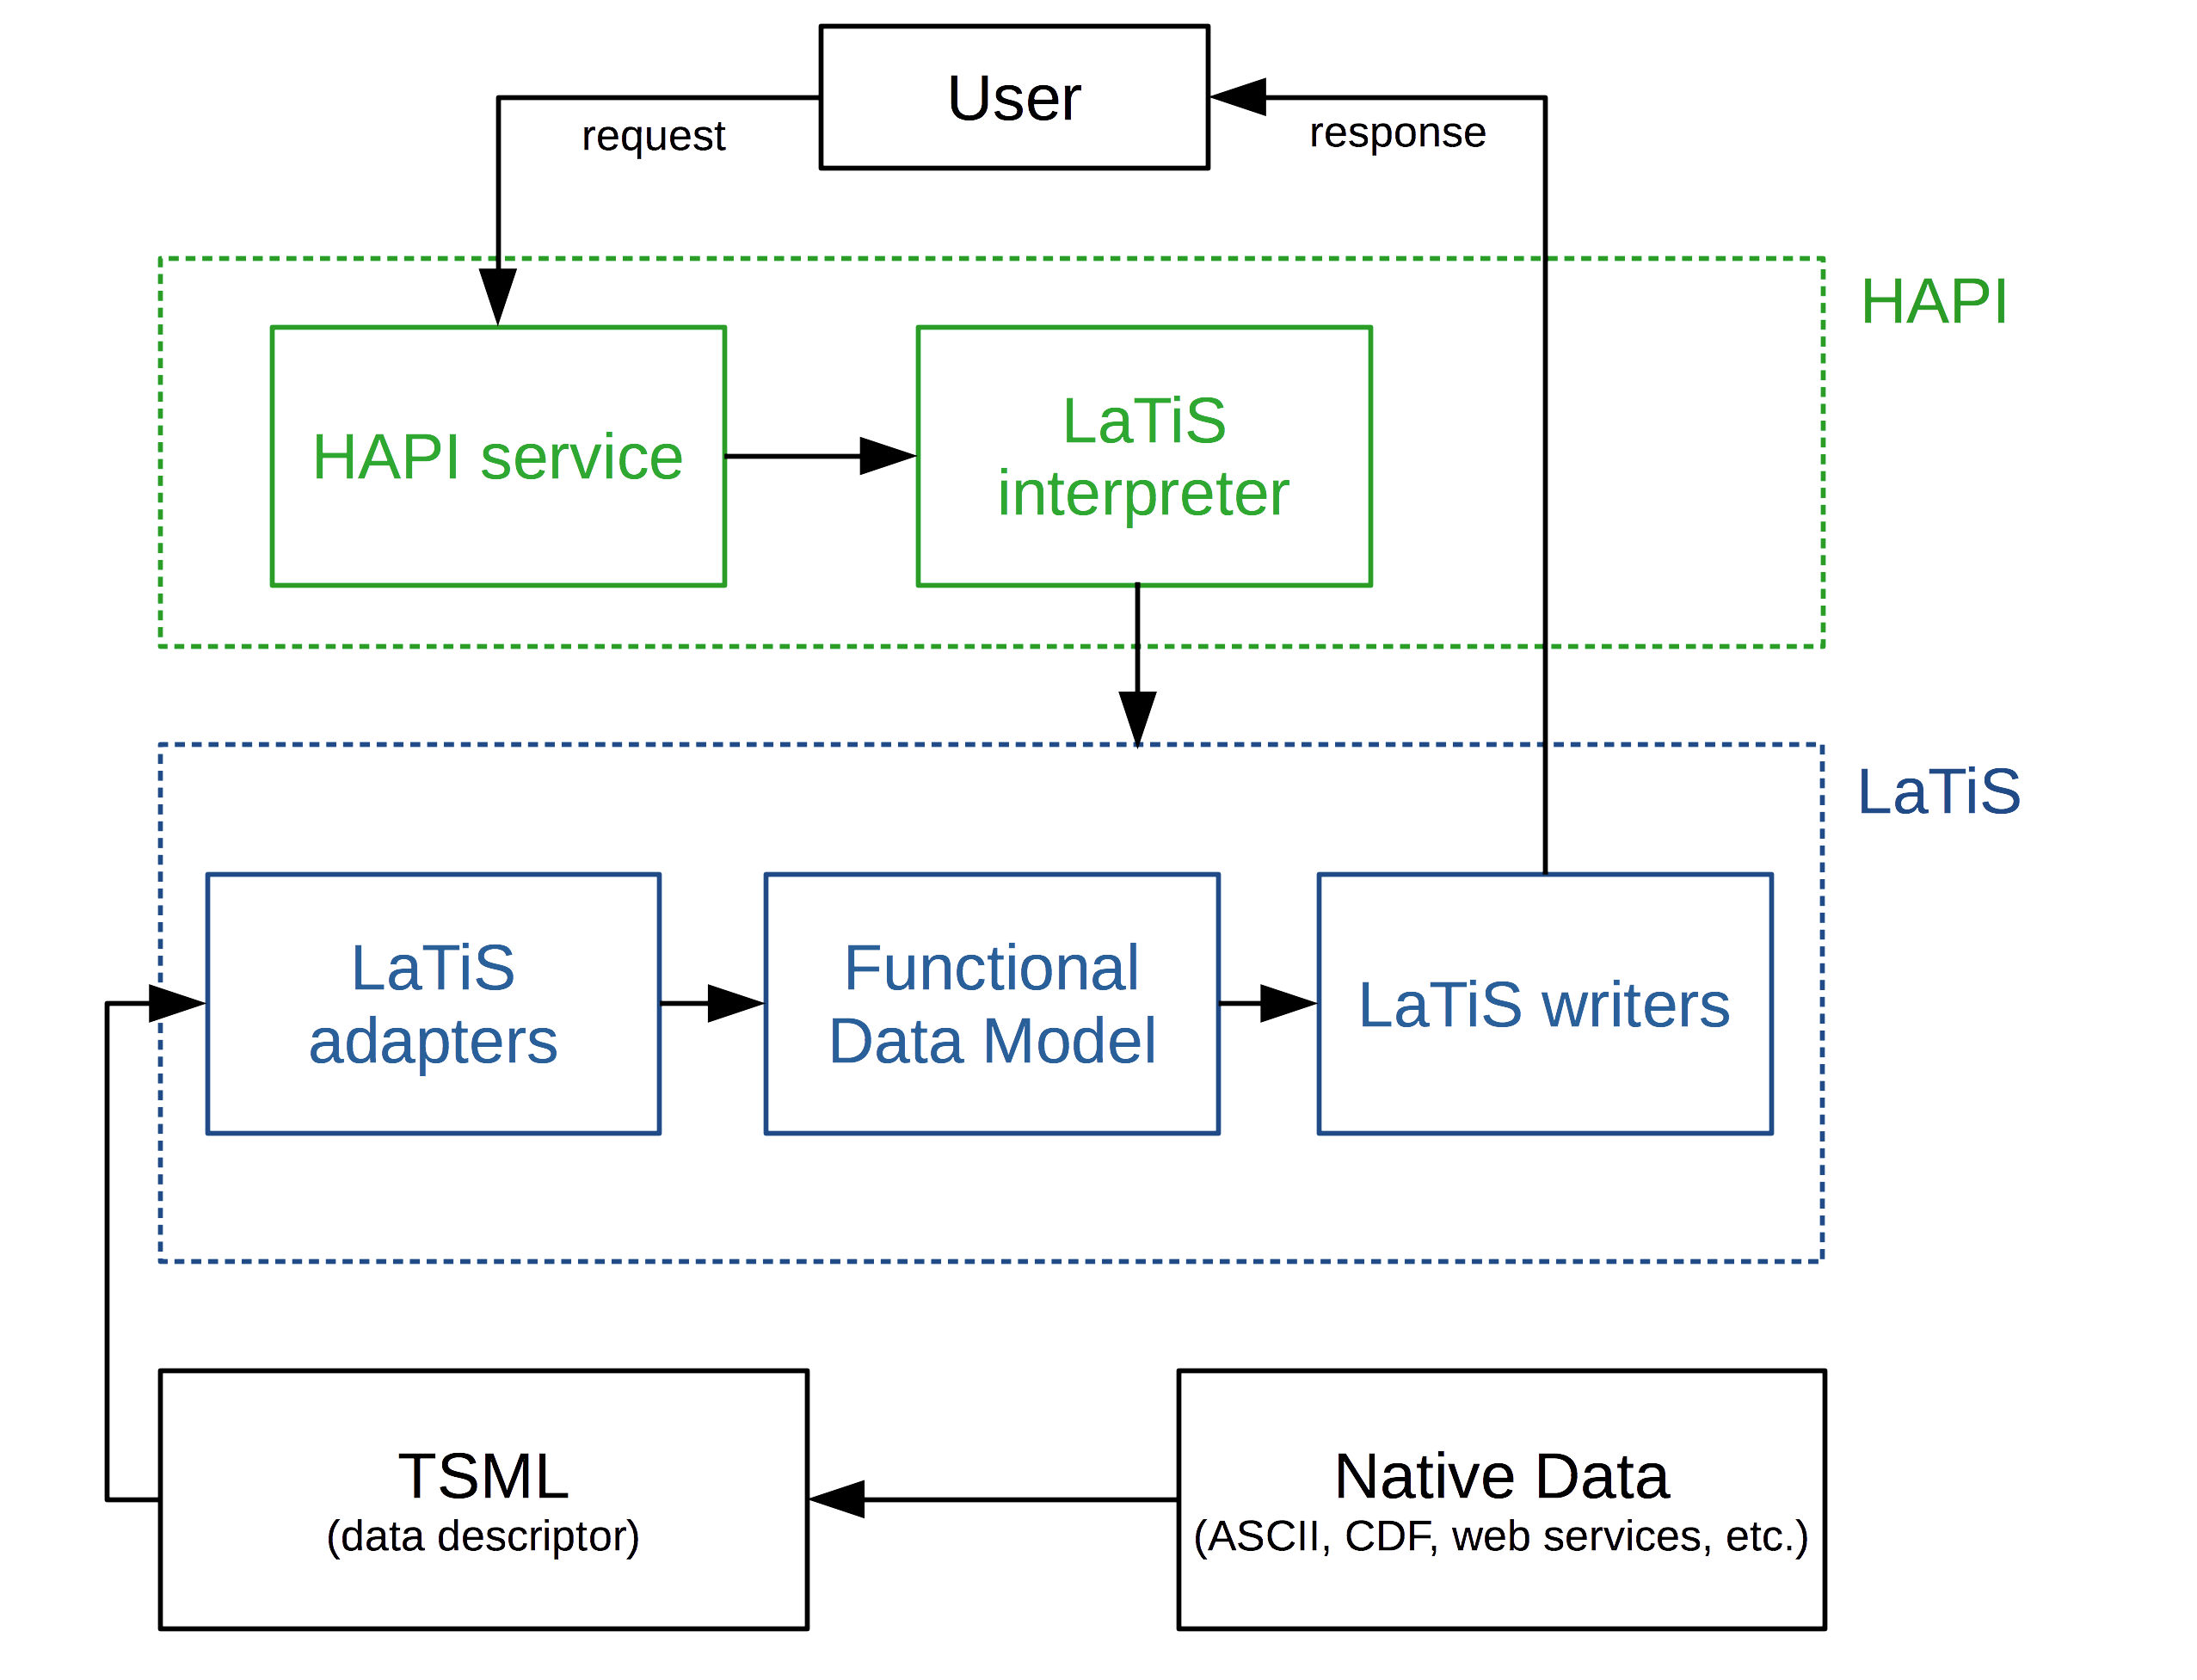
\includegraphics[scale=1.2]{img/flow}
        \end{tikzfigure}
      }

      \subcolumn{0.5}
      \block{}{
        \begin{tikzfigure}[Service architecture]
          \label{fig:fig1}
          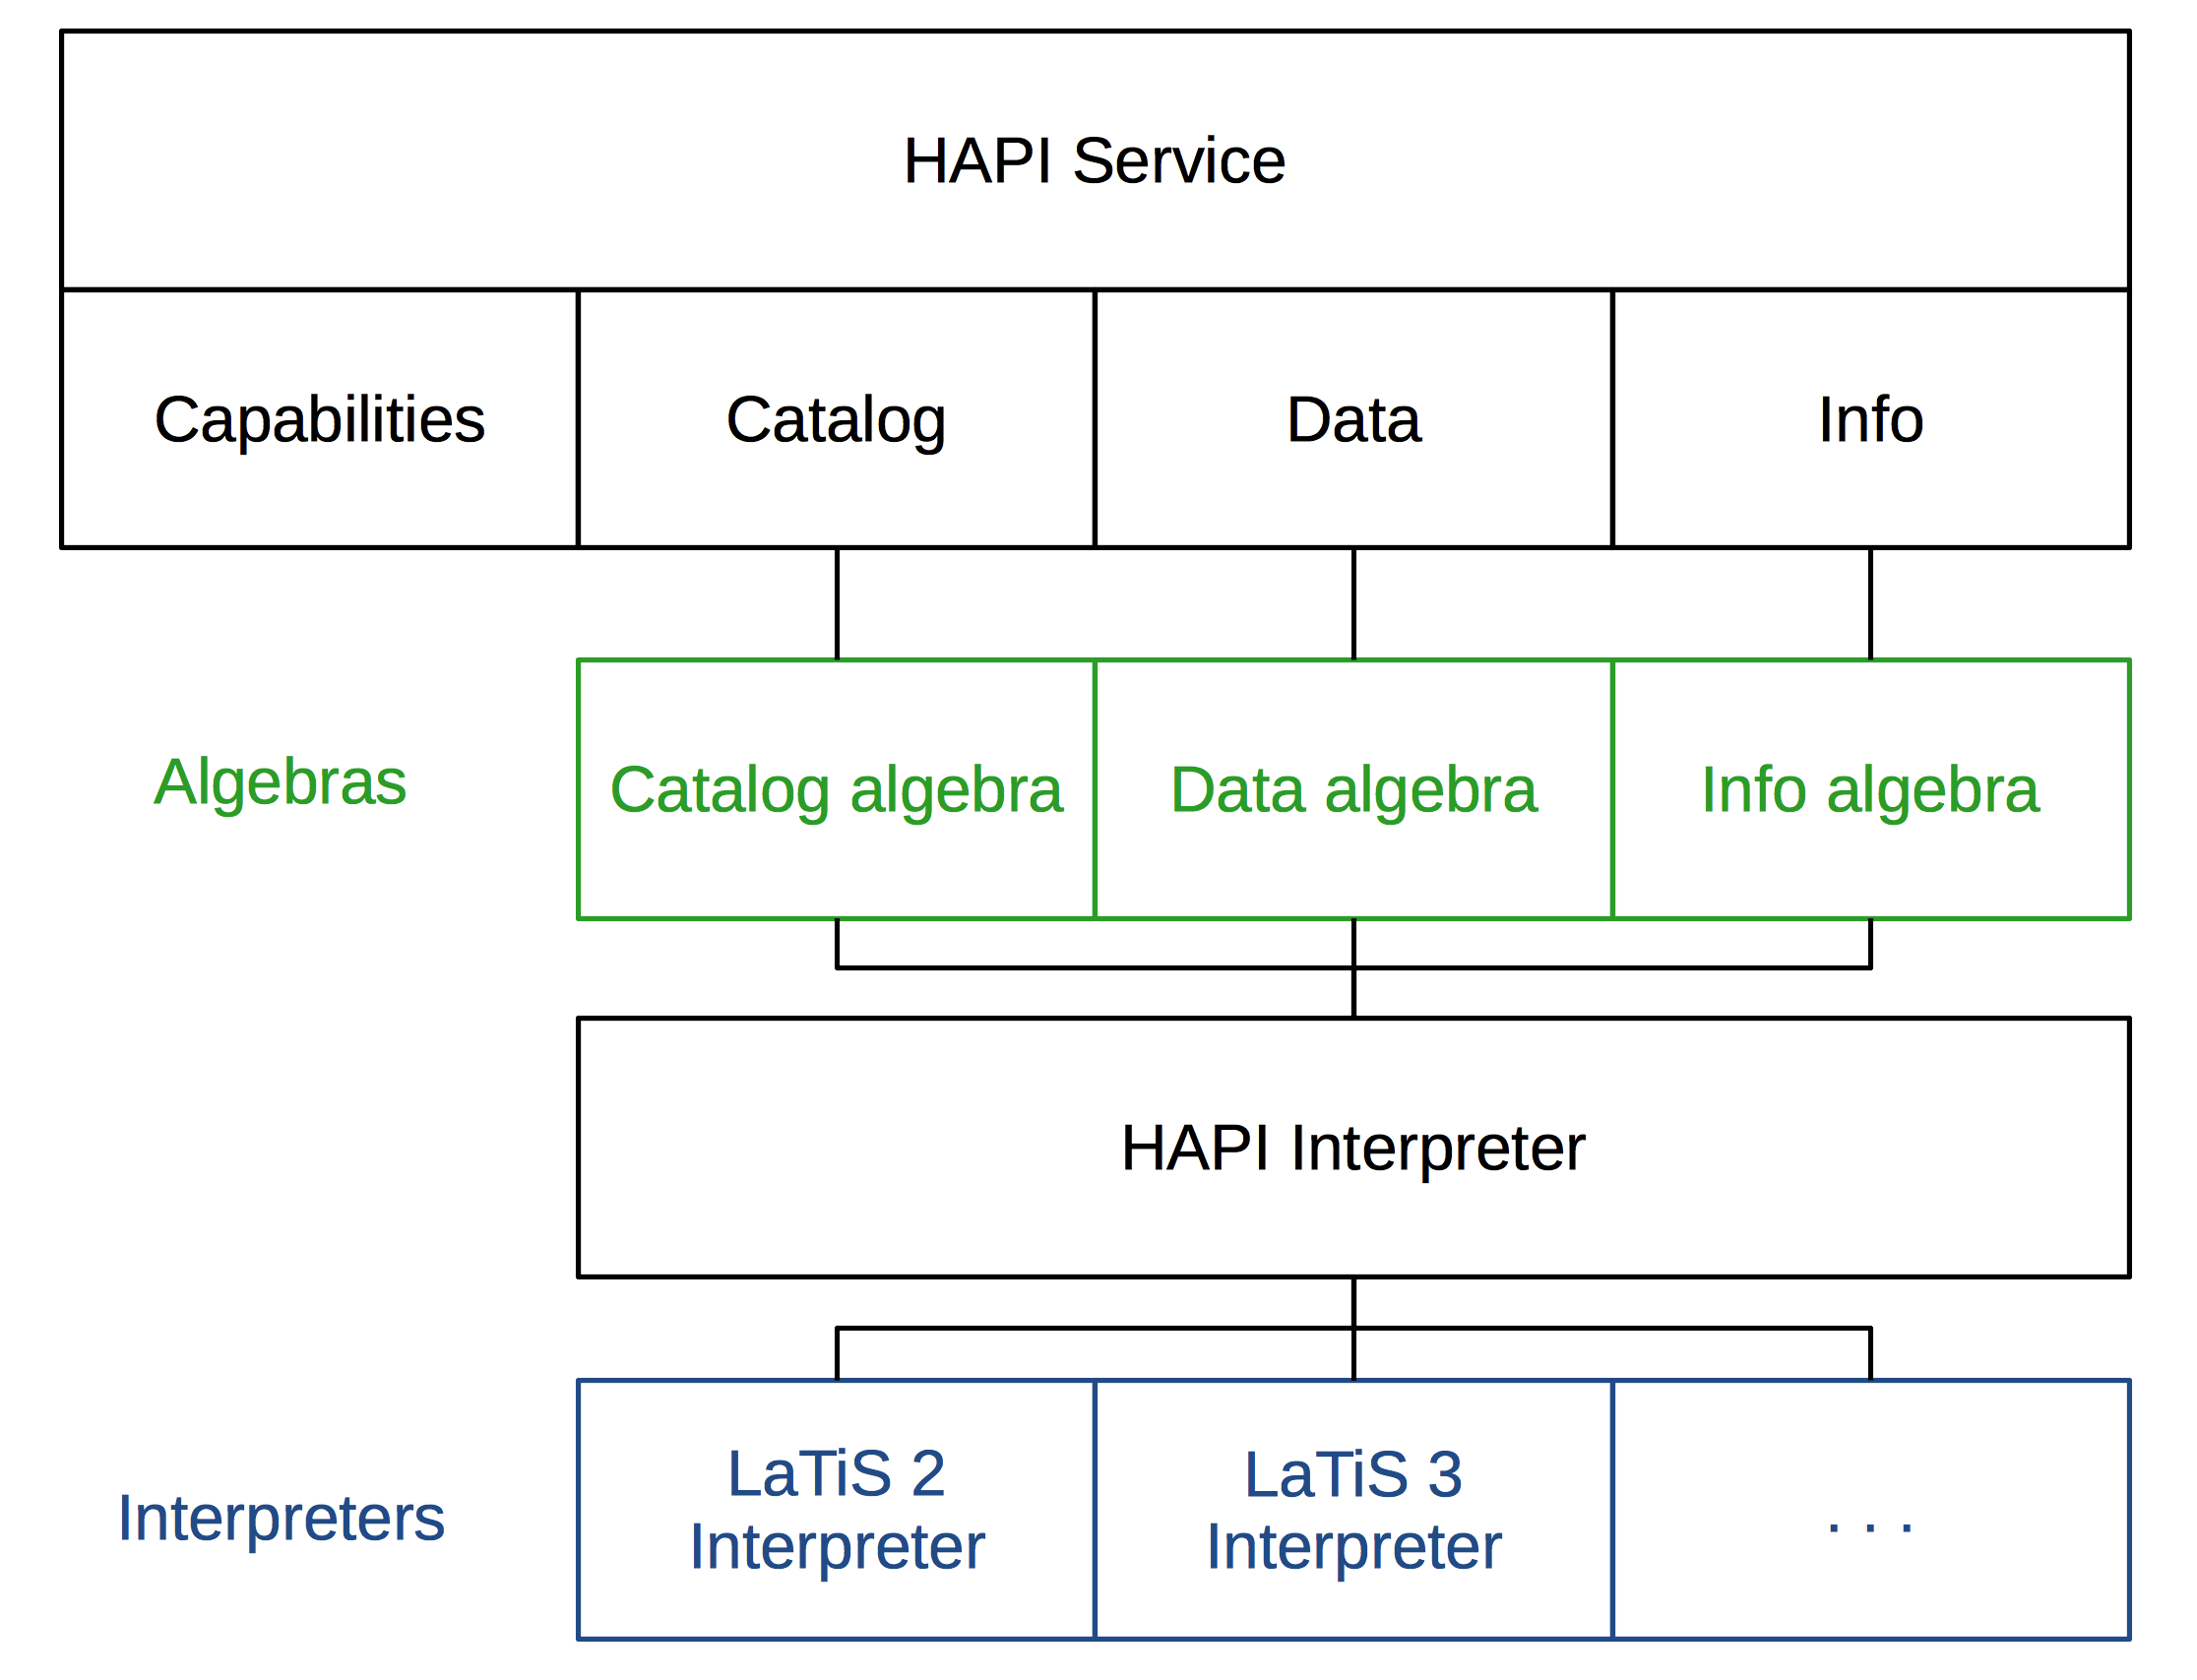
\includegraphics[scale=0.4]{img/architecture-diagram}
        \end{tikzfigure}
      }
    \end{subcolumns}

    \block{Server Implementation}{

      Our server is implemented in purely functional Scala using the
      \texttt{http4s} web framework. We implemented the server with a
      tagless final DSL (domain-specific language) to decouple generic
      server concerns from the data access layer. While LaTiS 2 is the
      default data access library, any library or service for which an
      interpreter can be defined may be used. \\

      \begin{minipage}[t]{0.45\linewidth}
        \setlength{\parskip}{0.5em}
        \section*{Algebras}
        Each HAPI endpoint is described by an algebra defining the
        operations provided by the endpoint. For instance, the
        \texttt{catalog} endpoint returns the catalog of datasets, so
        the catalog algebra defines an operation to get the catalog.

        \inputminted{scala}{src/Algebras.scala}

        The implementation of each endpoint is done in terms of the
        operations defined in the corresponding algebra. This way, we
        separate generic server concerns (e.g. routing, response
        formatting) from implementation-specific concerns (e.g. how to
        get a catalog).

        \inputminted[
          highlightlines=11,
          highlightcolor=yellow
        ]{scala}{src/Service.scala}
      \end{minipage}
      \hspace{0.1\linewidth}
      \begin{minipage}[t]{0.45\linewidth}
        \setlength{\parskip}{0.5em}
        \section*{Interpreters}
        Interpreters translate the DSL defined by the algebra to a
        specific implementation. The default interpreter uses the
        LaTiS 2 library.

        \inputminted{scala}{src/Interpreter1.scala}

        One can define other interpreters using other data access
        libraries or that used canned data for testing purposes.

        \inputminted{scala}{src/Interpreter2.scala}
      \end{minipage}
    }
  \end{columns}
\end{document}
